\chapter{DISEÑO MECÁNICO DEL SISTEMA}\label{cap:diseno-mecanico}
\listasdecapitulo{5}

El subsistema mecánico cumple una función operativa directa: condiciona la calidad del sensado de la cámara, la temperatura de la electrónica, la mantenibilidad del conjunto y la resistencia a manipulación y a las solicitaciones ambientales de Lima Metropolitana. Este capítulo desarrolla los requerimientos verificables, la presentación general y la selección de materiales, el sistema de movimiento de la cámara, el gabinete con su rack interno, el soporte del controlador semafórico, y la verificación estructural y térmica del conjunto. La cámara empleada es una cámara domo IP (tipo Hikvision) que opera con visión por computadora; el sistema de movimiento descrito tiene como único propósito orientar dicha cámara para optimizar la cobertura de la intersección.

\section{Requerimientos mecánicos verificables}\label{sec:requerimientos-mecanicos}

El gabinete y el soporte de cámara son subsistemas funcionales que deben demostrar su desempeño mediante CAD, cálculo, simulación por elementos finitos o especificación del fabricante. La Tabla~\ref{tab:requerimientos-mecanicos} concentra los criterios de diseño y el método de verificación asociado a cada uno.

\begin{table}[H]
  \centering
  \caption{Requerimientos mecánicos verificables del sistema.}
  \label{tab:requerimientos-mecanicos}
  \begin{tabularx}{\linewidth}{@{}l X X@{}}
    \toprule
    \textbf{Código} & \textbf{Criterio y objetivo de diseño} & \textbf{Verificación} \\
    \midrule
    RM-01 & Resistencia estructural: soportar peso propio, componentes, viento, vibración y acciones de mantenimiento. & Cargas, Von Mises, desplazamiento y factor de seguridad (Sección~\ref{sec:analisis-estructural}). \\
    RM-02 & Protección ambiental: grado IP objetivo, sellos y drenaje de condensación. & Especificación de gabinete y revisión de juntas. \\
    RM-03 & Manipulación/vandalismo: cerradura, tornillería protegida y material resistente. & Inspección CAD y análisis de puntos accesibles. \\
    RM-04 & Acceso de mantenimiento: sustitución de módulos sin desmontaje completo. & Secuencia de apertura y espacio de herramientas. \\
    RM-05 & Ventilación y temperatura: mantener componentes dentro de límites de hoja de datos. & Balance térmico y plan de validación experimental (Sección~\ref{sec:analisis-termico}). \\
    RM-06 & Expansión: reserva para terminales, comunicación o almacenamiento adicional. & Volumen libre y capacidad de riel/rack. \\
    RM-07 & Soporte de cámara: cobertura de zonas de interés con rigidez y torque suficientes. & Geometría de visión, cálculo de torque y desplazamiento (Sección~\ref{sec:movimiento-camara}). \\
    RM-08 & Material y corrosión: compatibilidad con humedad, radiación y mantenimiento urbano. & Matriz de materiales, acabado y vida útil propuesta. \\
    RM-09 & Peso e instalación: masa compatible con poste/estructura y procedimiento de montaje. & Presupuesto de masa y revisión del soporte existente. \\
    \bottomrule
  \end{tabularx}
  \fuente{Elaboración propia.}
\end{table}

\subsection{Requerimientos estructurales globales}\label{subsec:requerimientos-estructurales}

El sistema debe soportar las siguientes solicitaciones para garantizar funcionalidad y seguridad operativa.

\textbf{Cargas muertas.} El sistema soporta el peso del gabinete y módulo IoT con sus componentes internos (placa, microcontrolador, sensores, actuadores y estructura), el UPS y el controlador, los accesorios de comunicación (antenas y cámara) y el cableado eléctrico y de comunicaciones (MML, 2022). En particular, debe sostener la cámara domo como sensor principal de detección vehicular y el sistema de movimiento automatizado.

\textbf{Cargas ambientales.} Las cargas de viento se calculan según la NTE E.020 \emph{Cargas} del Reglamento Nacional de Edificaciones (SENCICO), norma de aplicación obligatoria para Lima Metropolitana, complementada con AASHTO LRFD para estructuras de soporte de señalización vial. Se adopta un periodo de retorno de 50 años y una presión de viento de diseño de 1.0~kPa (velocidad de referencia $\approx 145$~km/h); la verificación por elementos finitos (Sección~\ref{sec:analisis-estructural}) emplea además una condición extrema envolvente de 1.5~kPa ($\approx 175$~km/h).

\textbf{Cargas de temperatura.} Los criterios municipales establecen rangos operativos para equipamiento general (MML, 2022) y el Manual ITS del MTC exige resistencia a altas temperaturas, humedad, polvo y exposición solar (MTC, 2020). La normativa de la ATU es más restrictiva para equipos IoT con GPS, requiriendo operación entre $-20$\,°C y $+60$\,°C (ATU, 2024). Aplicando el criterio más restrictivo, se establece el rango de diseño de $-20$\,°C a $+60$\,°C.

\textbf{Rigidez y estabilidad.} El sistema debe limitar deflexiones para evitar problemas de serviciabilidad bajo carga muerta y resistir fatiga ante cargas cíclicas de viento y vibraciones de tráfico (MTC, 2020; MML, 2022).

\textbf{Protección contra corrosión.} Las estructuras metálicas requieren galvanización por inmersión en caliente según NTP-ISO 1461:2007 y acabado de poliuretano con resistencia UV, considerando el clima costero de Lima con alta humedad salina (MML, 2022).

\textbf{Vida útil.} El sistema semafórico debe tener una vida útil mínima de 120 meses; las estructuras metálicas y el gabinete, mínimo 15 años, con protección IP65/IK10 para la electrónica sensible (MML, 2022).

\subsection{Restricciones de diseño}\label{subsec:restricciones-diseno}

El gabinete se define en 800~mm $\times$ 600~mm $\times$ 500~mm (alto-ancho-profundidad). Como referencia, los gabinetes estándar NEMA TS-2 / ITE ATC presentan dimensiones aproximadas de 1\,245~mm $\times$ 762~mm $\times$ 432~mm (formato ``M''); el diseño propuesto conserva sus criterios funcionales de distribución interna con una reducción volumétrica optimizada a los componentes alojados. El sistema debe operar con humedad relativa de hasta 90~\%, resistir corrosión salina, soportar radiación UV directa y cumplir un grado de protección mínimo IP65 (MML, 2022), protección mecánica anti-vandálica IK10, ventilación forzada activada a 40\,°C y los requisitos de transmisión en tiempo real del SIT-ATU (ATU, 2024).

\section{Presentación general del sistema y materiales}\label{sec:presentacion-materiales}

El sistema mecánico integra cuatro subsistemas: el gabinete de aluminio 5052-H32 (masa $\approx 21.98$~kg); el rack interno de soporte que aloja toda la electrónica (masa $\approx 11.965$~kg con componentes); el sistema de movimiento angular de la cámara (masa $\approx 3.5$~kg, que incluye motor paso a paso NEMA~23, biela, conector de aluminio y rodamiento de Ø120~mm) montado sobre un aro estructural giratorio de 7.8~kg; y el conjunto de visión con cámara domo y soporte (0.65~kg). La masa total del sistema completo es de 47.126~kg ($\approx 47$~kg), distribuida para optimizar la estabilidad estructural y facilitar la instalación y el mantenimiento. Las Figuras~\ref{fig:sistema-interseccion} y~\ref{fig:sistema-completo} presentan el conjunto en su posición de operación en una intersección vehicular.

\begin{figure}[H]
  \centering
  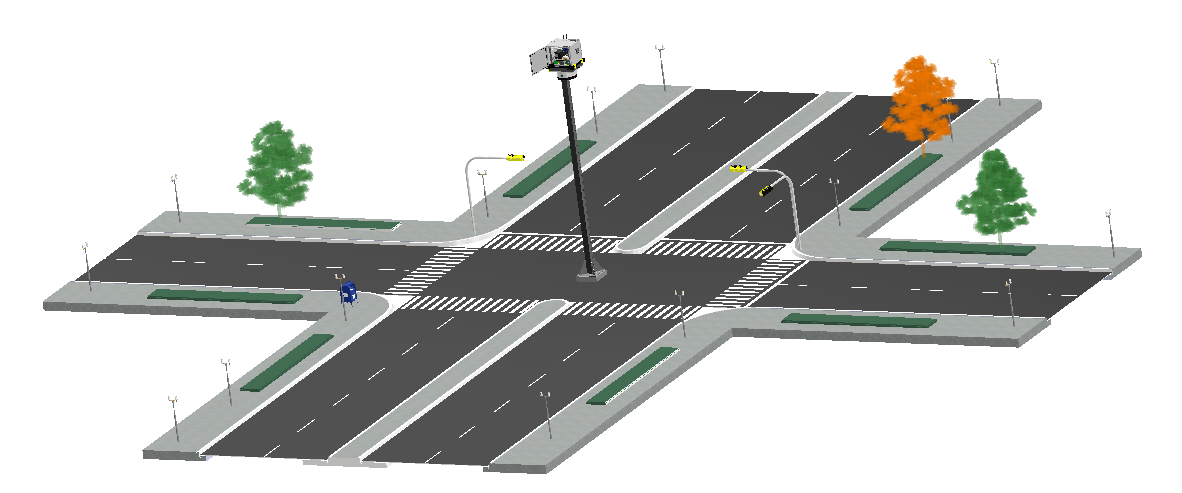
\includegraphics[width=0.8\linewidth,keepaspectratio]{media/image30.png}
  \caption{Vista del controlador semafórico instalado en una intersección vehicular.}
  \label{fig:sistema-interseccion}
  \fuente{Elaboración propia.}
\end{figure}

\begin{figure}[H]
  \centering
  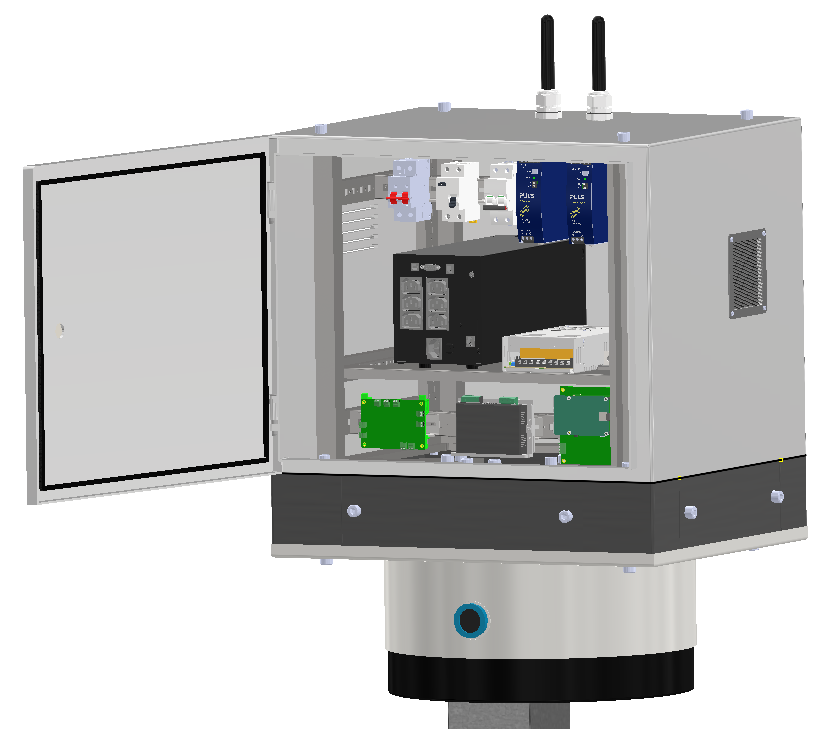
\includegraphics[width=0.8\linewidth,keepaspectratio]{media/image64.png}
  \caption{Vista general del controlador semafórico propuesto.}
  \label{fig:controlador-vista}
  \fuente{Elaboración propia.}
\end{figure}

\begin{figure}[H]
  \centering
  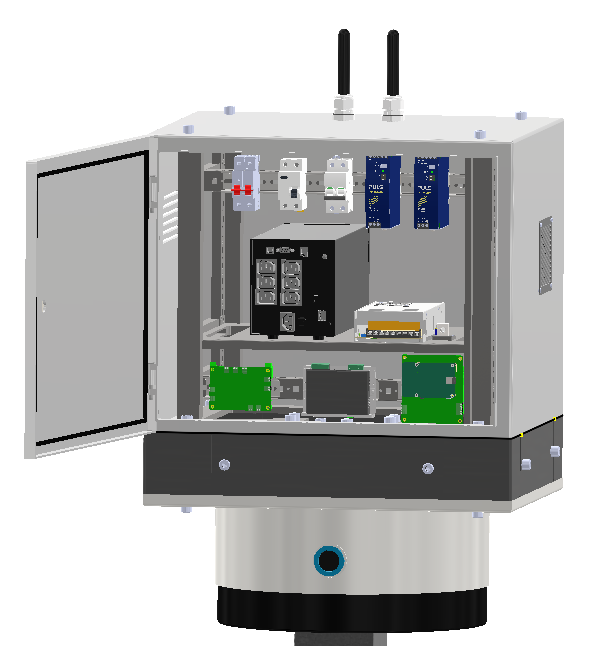
\includegraphics[width=0.8\linewidth,keepaspectratio]{media/image111.png}
  \caption{Sistema completo ensamblado (sin poste de soporte).}
  \label{fig:sistema-completo}
  \fuente{Elaboración propia.}
\end{figure}

\subsection{Masa y centro de masa del sistema}\label{subsec:masa-centro-masa}

El análisis de masa y centro de gravedad es prioritario para garantizar la estabilidad estructural del gabinete y dimensionar el anclaje al poste. Se calculan las propiedades másicas de los tres componentes principales: el gabinete exterior, el rack interno con su electrónica, y el sistema de cámara con su mecanismo de movimiento.

\textbf{Gabinete.} Presenta una geometría de cubo hueco sin base inferior (Figura~\ref{fig:gabinete-vacio}), con dimensiones exteriores de 479~mm de altura, 600~mm de ancho y 525~mm de profundidad. Se fabrica en aluminio 5052-H32 con espesor de pared de 6~mm, que aporta rigidez frente a viento e impactos vandálicos (IK10) y resistencia a la corrosión salina. Considerando una densidad de 2\,680~kg/m\textsuperscript{3}, el volumen de material se obtiene por diferencia entre el volumen exterior e interior:

\begin{figure}[H]
  \centering
  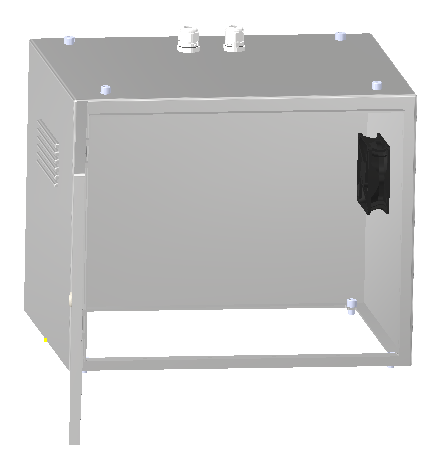
\includegraphics[width=0.8\linewidth,keepaspectratio]{media/image109.png}
  \caption{Gabinete sin componentes internos.}
  \label{fig:gabinete-vacio}
  \fuente{Elaboración propia.}
\end{figure}

\begin{equation}
V_{\text{ext}} = 0.479 \times 0.600 \times 0.525 = 0.1509~\text{m}^3
\end{equation}
\begin{equation}
V_{\text{int}} = 0.473 \times 0.588 \times 0.513 = 0.1427~\text{m}^3
\end{equation}
\begin{equation}
V_{\text{material}} = 0.1509 - 0.1427 = 0.0082~\text{m}^3
\end{equation}
\begin{equation}
m_{\text{gabinete}} = 2\,680 \times 0.0082 = 21.976~\text{kg}
\end{equation}

La ausencia de base inferior eleva ligeramente el centro de gravedad respecto al centro geométrico: en ancho se ubica a 300~mm (por simetría), en altura a $\approx 250$~mm desde la base (frente a los 239.5~mm del centro geométrico) y en profundidad a 262.5~mm desde el borde frontal.

\textbf{Rack interno.} El rack (Figura~\ref{fig:rack-completo}) soporta la electrónica y mide 466~mm $\times$ 440~mm $\times$ 539~mm. Su distribución vertical ubica los componentes más pesados en la base para reducir el centro de gravedad. La estructura de aluminio con perfiles de 30$\times$30~mm y bandejas perforadas se estima en 5.700~kg; sumando todos los componentes electrónicos, cableado, antenas y el sistema de ventilación, la masa total del rack resulta en 11.965~kg. Las masas individuales provienen de las fichas de fabricante (p.~ej. Raspberry~Pi~5: 0.075~kg; HAT~4G~LTE: 0.050~kg; driver DM542T: 0.350~kg; UPS~500\,VA: 3.500~kg; SMPS S-360-24: 1.200~kg). El centro de masa del rack se estima a 220~mm desde el borde posterior, 180~mm desde la base y 250~mm respecto al centro del ancho.

\begin{figure}[H]
  \centering
  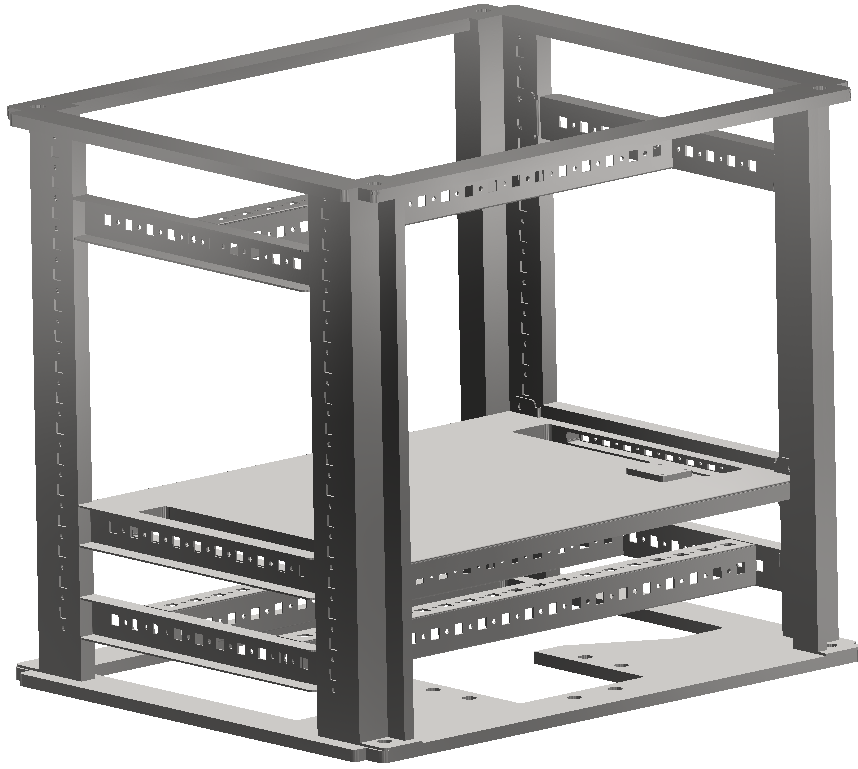
\includegraphics[width=0.8\linewidth,keepaspectratio]{media/image145.png}
  \caption{Rack interno completo de soporte de la electrónica.}
  \label{fig:rack-completo}
  \fuente{Elaboración propia.}
\end{figure}

\textbf{Sistema de cámara.} El conjunto de visión está constituido por una cámara domo IP (0.600~kg) montada sobre un soporte de aluminio (0.050~kg), totalizando 0.650~kg. Se posiciona en la parte móvil del sistema, sobre el aro giratorio, permitiendo un desplazamiento angular de 180° para optimizar el campo de visión. Su ubicación inferior reduce el momento de vuelco del conjunto y minimiza la longitud de cableado hacia el rack. Dado que representa solo el 1.38~\% de la masa total y su brazo de palanca respecto al eje del poste es reducido, su contribución al centro de masa global es despreciable en cálculos preliminares de estabilidad.

\textbf{Masa total y centro de masa global.} La masa total se obtiene sumando todas las contribuciones:

\begin{equation}
m_{\text{total}} = m_{\text{gabinete}} + m_{\text{rack}} + m_{\text{aro}} + m_{\text{mov}} + m_{\text{accesorios}} = 47.126~\text{kg}
\end{equation}

Definiendo el origen en la esquina inferior posterior izquierda del gabinete (eje $X$ hacia el frente, $Y$ hacia arriba, $Z$ lateral), el centro de masa global ponderado por las masas de gabinete, rack y cámara resulta:

\begin{equation}
X_{cm} = 273.2~\text{mm}, \qquad Y_{cm} = 223.9~\text{mm}, \qquad Z_{cm} = 254.9~\text{mm}
\end{equation}

El centro de masa se desplaza ligeramente hacia el frente por la concentración de electrónica, queda por debajo del centro vertical por el peso del UPS y la SMPS en la base, y se mantiene prácticamente centrado en dirección lateral por simetría. Esta ubicación justifica posicionar el punto de apoyo del poste a 110~mm desde el frente del gabinete, lo que minimiza los momentos de vuelco ante viento, reduce las tensiones en las uniones gabinete-poste y facilita el ruteo de cables. Los datos másicos detallados de cada componente se consignan en el Anexo correspondiente.

\subsection{Criterios de selección de materiales}\label{subsec:seleccion-materiales}

La selección de materiales atiende los requisitos normativos, las condiciones ambientales costeras de Lima y la durabilidad exigida. Se selecciona la aleación de aluminio 5052-H32 para el gabinete por su resistencia a la corrosión en atmósferas marinas y urbanas, su buena soldabilidad y su conformabilidad (Atlas, 2021; ThomasNet, 2025). Aunque la norma NEMA TS-2 establece los requisitos funcionales y ambientales de los gabinetes de control de tráfico sin imponer un material específico (NEMA, 2021), el 5052-H32 cumple holgadamente esos niveles de desempeño y el grado de protección IP65. Su contenido de magnesio (2.2--2.8~\%) y cromo (0.15--0.35~\%) le confiere grado marino, adecuado para la intemperie salina.

Frente al acero galvanizado, el aluminio 5052-H32 reduce el peso en $\approx 65$~\%, lo que facilita la instalación y disminuye los esfuerzos sobre la estructura de soporte; ofrece alta resistencia a la corrosión salina sin galvanización y elevada conductividad térmica (138~W/m·K), favoreciendo la disipación del calor interno (Atlas, 2021; MatWeb, 2024). Frente al policarbonato reforzado, aporta mayor rigidez estructural ante impactos y vibraciones, mejor disipación térmica, mayor durabilidad bajo radiación UV (vida útil estimada superior a 15 años, frente a 12 del policarbonato) y facilidad de conexión a tierra eléctrica (Wevolver, 2025). El acabado superficial es anodizado tipo II de 10--25~µm, que incrementa la resistencia a la corrosión y al desgaste, garantizando una vida útil superior a 10 años en servicio exterior continuo. Los materiales del poste (acero ASTM A36) y de la cimentación (hormigón armado) se justifican en la Sección~\ref{sec:soporte-controlador}.

\section{Sistema de movimiento de la cámara}\label{sec:movimiento-camara}

El sistema de posicionamiento angular permite un desplazamiento de 180° de la cámara mediante un mecanismo de biela-manivela acoplado a un rodamiento rígido de bolas, buscando maximizar la estabilidad y minimizar las vibraciones que afecten la captura de imágenes. Una biela de 150~mm conectada al eje del motor paso a paso NEMA~23 transmite el movimiento a la pista interior de un rodamiento de Ø120~mm; la cámara domo y su soporte se montan sobre dicha pista móvil. La configuración de apoyo bilateral distribuye el peso del conjunto cámara-soporte entre dos puntos, de modo que el motor prácticamente no genera torque para soportar cargas gravitatorias, destinándose su potencia a vencer la fricción residual y las fuerzas inerciales. Las Figuras~\ref{fig:camara-biela} a~\ref{fig:rodamiento-motor} muestran el mecanismo.

\begin{figure}[H]
  \centering
  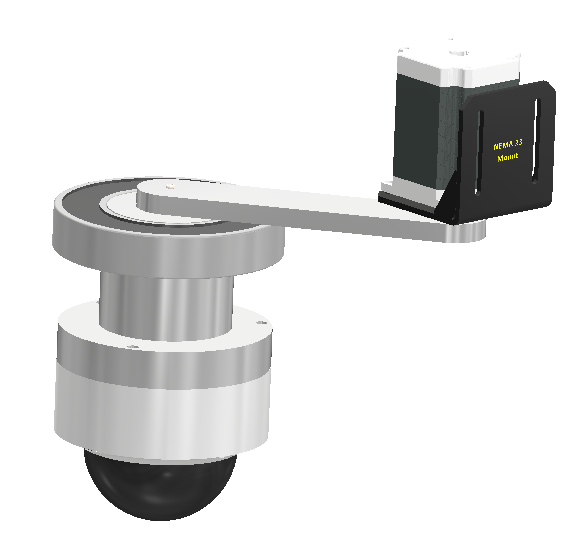
\includegraphics[width=0.8\linewidth,keepaspectratio]{media/image42.png}
  \caption{Conjunto cámara domo, soporte y biela de transmisión.}
  \label{fig:camara-biela}
  \fuente{Elaboración propia.}
\end{figure}

\begin{figure}[H]
  \centering
  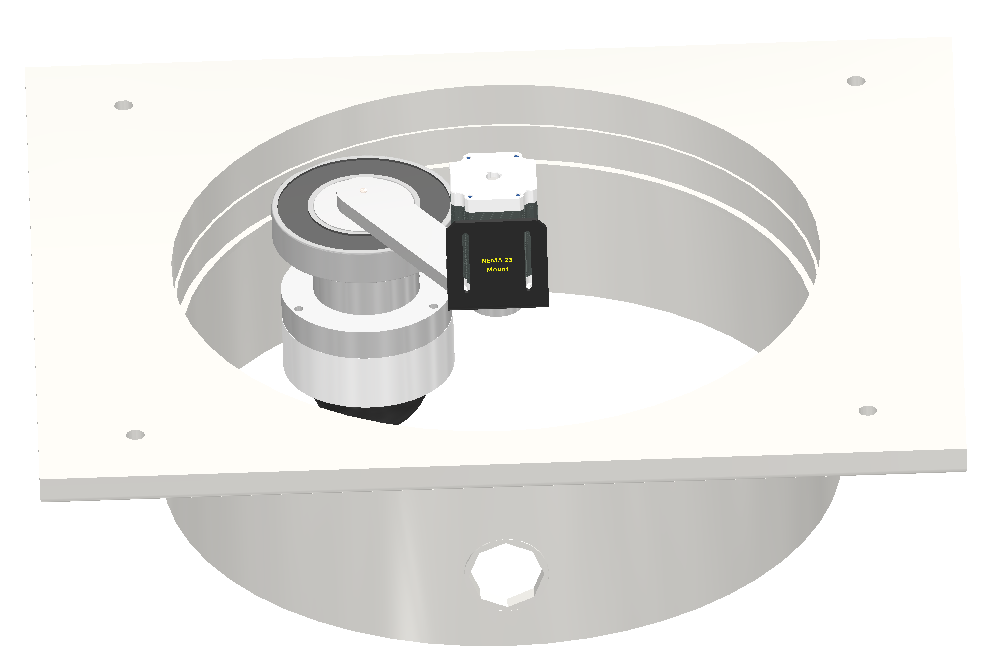
\includegraphics[width=0.8\linewidth,keepaspectratio]{media/image37.png}
  \caption{Vista del aro de giro y el rodamiento de Ø120~mm.}
  \label{fig:aro-rodamiento}
  \fuente{Elaboración propia.}
\end{figure}

\begin{figure}[H]
  \centering
  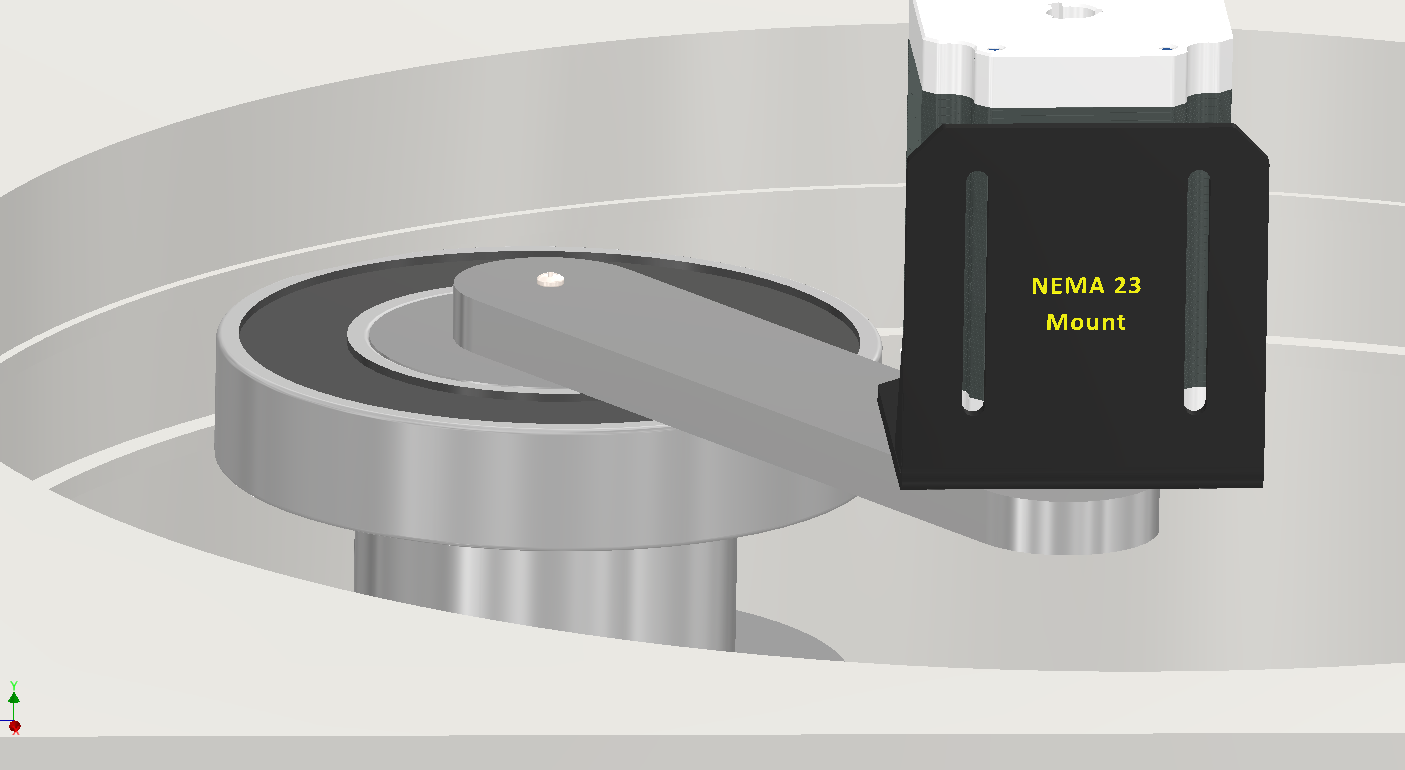
\includegraphics[width=0.8\linewidth,keepaspectratio]{media/image51.png}
  \caption{Vista del rodamiento, la biela y el motor paso a paso.}
  \label{fig:rodamiento-motor}
  \fuente{Elaboración propia.}
\end{figure}

\subsection{Diagrama de cuerpo libre y datos del mecanismo}\label{subsec:dcl-movimiento}

El análisis parte del diagrama de cuerpo libre (DCL) del sistema de vigilancia (Figura~\ref{fig:dcl}), que representa las fuerzas actuantes: los pesos del motor ($W_m$), la biela ($W_b$), el aro estructural ($W_a$), el soporte ($W_s$), la cámara ($W_c$) y el rodamiento ($W_r$); las reacciones en la sujeción al gabinete ($G_x$, $G_y$); la fuerza normal transmitida por la biela ($B$); las normales de reacción ($N$, $N_s$, $N_{C1}$, $N_{C2}$); la fricción del rodamiento ($F_R$) y el torque del motor ($T$).

\begin{figure}[H]
  \centering
  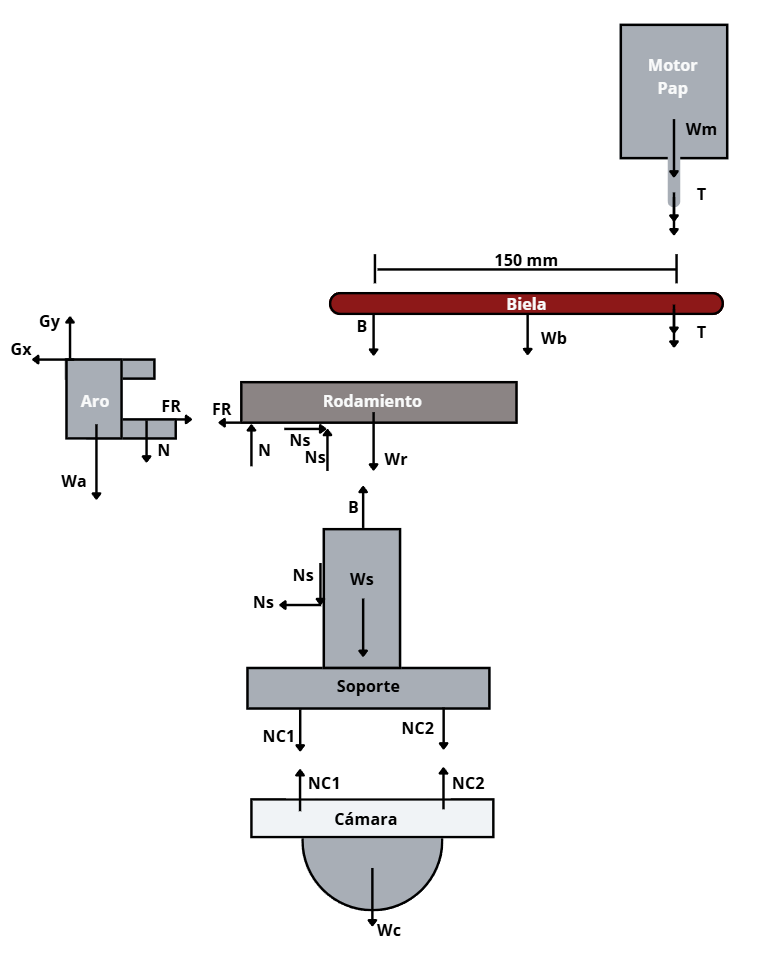
\includegraphics[width=0.8\linewidth,keepaspectratio]{media/image125.png}
  \caption{Diagrama de cuerpo libre del sistema de vigilancia.}
  \label{fig:dcl}
  \fuente{Elaboración propia.}
\end{figure}

Los datos relevantes del mecanismo son: rodamiento rígido de bolas sellado de Ø120~mm (radio medio $r = 60$~mm, coeficiente de fricción $\mu = 0.002$); biela de aluminio 5052-H32 de 150~mm de longitud, 35~mm de ancho y 10~mm de espesor (área transversal $A = 350$~mm\textsuperscript{2}); conector cámara-biela de aluminio mecanizado (0.857~kg); aro estructural de aluminio 5052-H32 (7.800~kg); conjunto cámara más soporte ($m = 0.650$~kg, peso $W_c + W_s = 6.38$~N); y motor NEMA~23 con torque nominal de 1.8~N·m y masa de 1.500~kg.

El equilibrio vertical del aro arroja una reacción $G_y \approx 92.71$~N y una reacción horizontal $G_x \approx 0.29$~N (despreciable con $\theta \approx 0^\circ$). La cámara se apoya en dos puntos de contacto que, por simetría, reparten la carga: $N_{C1} = N_{C2} = 3.19$~N. La carga normal total sobre el rodamiento es $W_a + W_r + W_s + W_c = 92.71$~N, de modo que la fuerza de fricción y el torque resistivo asociado resultan:

\begin{equation}
F_R = \mu \times 92.71 = 0.002 \times 92.71 = 0.185~\text{N}
\end{equation}
\begin{equation}
T_{\text{fricción}} = F_R \times r = 0.185 \times 0.060 = 0.011~\text{N·m} = 11~\text{mN·m}
\end{equation}

\subsection{Verificación del motor paso a paso seleccionado}\label{subsec:verificacion-motor}

El motor paso a paso NEMA~23 fue seleccionado en el Capítulo~\ref{cap:diseno-electronico} con un torque nominal disponible de 1.8~N·m. Esta sección verifica que dicho torque supera el torque requerido por el mecanismo en su condición de dimensionamiento más desfavorable. Adoptando el requerimiento de torque establecido en el dimensionamiento, $T_{\text{req}} \approx 0.591$~N·m, la verificación se cierra comparándolo con el torque disponible:

\begin{equation}
T_{\text{disp}} = 1.8~\text{N·m} \;>\; T_{\text{req}} \approx 0.591~\text{N·m}
\end{equation}
\begin{equation}
FS_{\text{motor}} = \frac{T_{\text{disp}}}{T_{\text{req}}} = \frac{1.8}{0.591} \approx 3.05
\end{equation}

El motor satisface el requerimiento con un factor de seguridad de $\approx 3.0$, suficiente para una operación sin pérdida de pasos. La demanda de torque \emph{operativa} real del mecanismo optimizado es aún menor: considerando un factor de seguridad de dimensionamiento $FS = 2.0$ sobre el peso del conjunto de visión y una aceleración angular conservadora $\alpha = 0.5$~rad/s\textsuperscript{2} con momento de inercia $I \approx 0.012$~kg·m\textsuperscript{2}, las contribuciones de fricción e inercia son:

\begin{equation}
T_{\text{fricción}} = \mu \times W_{\text{diseño}} \times r = 0.002 \times 12.76 \times 0.060 \approx 1.53~\text{mN·m}
\end{equation}
\begin{equation}
T_{\text{inercial}} = I \times \alpha = 0.012 \times 0.5 = 6~\text{mN·m}
\end{equation}
\begin{equation}
T_{\text{dinámico}} = T_{\text{fricción}} + T_{\text{inercial}} = 1.53 + 6 = 7.53~\text{mN·m}
\end{equation}

Por tanto, el apoyo bilateral del rodamiento reduce la demanda operativa a $\approx 7.5$~mN·m, muy por debajo tanto del requerimiento de dimensionamiento (0.591~N·m) como del torque nominal (1.8~N·m). Ambas comprobaciones confirman la idoneidad del motor seleccionado, con un margen amplio frente a cargas imprevistas o condiciones ambientales adversas.

\subsection{Análisis estructural de la biela}\label{subsec:analisis-biela}

La biela transmite el movimiento mediante un esfuerzo predominantemente de tracción-compresión alternante. Para el caso crítico (biela horizontal), la fuerza axial máxima teórica es $B = T_{\text{motor}}/r_{\text{biela}} = 1.8/0.150 = 12$~N. Dado que la demanda operativa real es muy inferior, la fuerza efectiva en la biela, afectada por el factor de seguridad, es del orden de $F_{\text{biela}} \approx 0.1$~N, lo que produce una tensión:

\begin{equation}
\sigma_{\text{biela}} = \frac{F_{\text{biela}}}{A} = \frac{0.1~\text{N}}{350~\text{mm}^2} = 2.86 \times 10^{-4}~\text{MPa}
\end{equation}

Con las propiedades del aluminio 5052-H32 (resistencia a tracción 228~MPa, módulo de elasticidad 70\,300~MPa, límite elástico 193~MPa, resistencia a fatiga a $10^7$ ciclos 117~MPa), el factor de seguridad del material es extremadamente alto ($\approx 8 \times 10^5$), con una utilización inferior al 0.0002~\%. La biela presenta así vida prácticamente infinita a fatiga; su dimensionamiento está dominado por consideraciones geométricas de acoplamiento mecánico con el motor y el rodamiento, no por resistencia. La reacción vertical $G_y = 92.71$~N se distribuye entre los puntos de fijación del aro al gabinete mediante tornillería M12, con cargas individuales del orden de 10--15~N por tornillo, plenamente manejables.

\section{Gabinete y soporte tipo rack}\label{sec:gabinete-rack}

El gabinete principal de aluminio 5052-H32 (21.976~kg) aloja toda la electrónica mediante un rack interno de soporte (5.700~kg de estructura, 11.965~kg con componentes), fabricado con perfiles de aluminio de 30$\times$30~mm y bandejas perforadas que permiten organización modular, facilitan el mantenimiento y optimizan la gestión térmica.

\subsection{Arquitectura de distribución vertical en el rack}\label{subsec:arquitectura-rack}

El rack mide 466~mm $\times$ 440~mm $\times$ 539~mm y emplea rieles DIN estándar que aportan flexibilidad para futuras expansiones. La masa total con componentes montados es de 11.965~kg, distribuida en cuatro niveles funcionales según criterios de funcionalidad, accesibilidad, disipación térmica y seguridad eléctrica (Figura~\ref{fig:rack-componentes}).

\begin{itemize}
  \item \textbf{Nivel 1 (superior) -- Protección eléctrica:} breaker termomagnético Schneider C60N-C6 (6~A), RCD Schneider ID~K 25\,A/30\,mA (desconexión $<30$~ms) y DPS Phoenix Contact VAL-MS~230 (limita sobretensiones a $<1.5$~kV). Se ubican arriba para facilitar inspecciones.
  \item \textbf{Nivel 2 (intermedio-superior) -- Alimentación y conversión:} SMPS S-360-24 (220~V~AC a 24~V~DC, 15~A/360~W, eficiencia 85~\%, disipación 63.5~W) y dos conversores DC-DC LM2596 (5~V/3~A y 12~V/2~A). Próximos a las rejillas de ventilación superior.
  \item \textbf{Nivel 3 (intermedio-inferior) -- Respaldo energético:} UPS 500\,VA con baterías VRLA 12~V/7~Ah en serie (24~V), respaldo de 15--20~min y conmutación $<10$~ms. Por ser el componente más pesado (3.5~kg), contribuye a mantener bajo el centro de masa.
  \item \textbf{Nivel 4 (inferior) -- Procesamiento, control y actuación:} PCB controladora con Raspberry~Pi~5 y HAT~4G~LTE Quectel EG25-G (0.175~kg), driver DM542T (16 micropasos, 3.0~A) y PCB de distribución de voltaje (100$\times$70~mm, FR-4). Incluye la instrumentación: sensor de corriente WCS1600, sensor ultrasónico URM06 RS485 y sensor de temperatura DS18B20.
\end{itemize}

\begin{figure}[H]
  \centering
  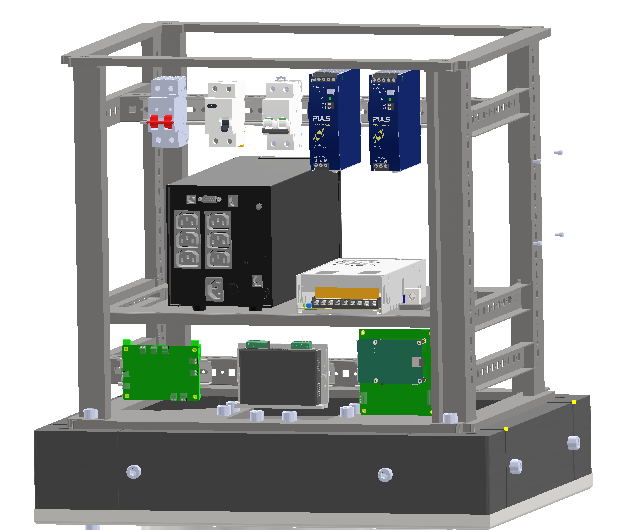
\includegraphics[width=0.8\linewidth,keepaspectratio]{media/image73.png}
  \caption{Rack con todos sus componentes electrónicos montados.}
  \label{fig:rack-componentes}
  \fuente{Elaboración propia.}
\end{figure}

\section{Soporte del controlador semafórico}\label{sec:soporte-controlador}

El soporte fija el gabinete a 4.8~m de altura sobre el nivel del terreno mediante un poste tubular de acero (Figura~\ref{fig:conexion-poste}). El peso total del gabinete genera una carga vertical de $W = 47.126 \times 9.81 = 462$~N; sin embargo, para el análisis estructural se adopta una carga simplificada conservadora de 35~kg ($\approx 350$~N), considerando que parte de la masa corresponde a componentes removibles durante el mantenimiento.

\begin{figure}[H]
  \centering
  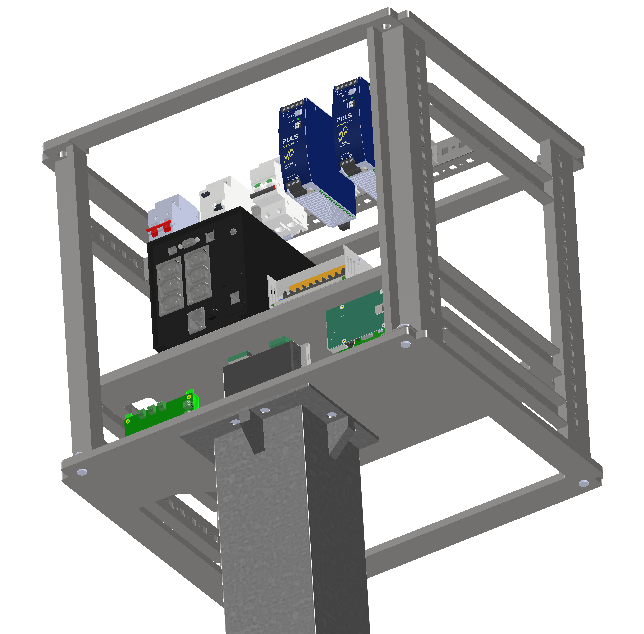
\includegraphics[width=0.8\linewidth,keepaspectratio]{media/image104.png}
  \caption{Conexión entre el rack/gabinete y el poste de acero de sección cuadrada.}
  \label{fig:conexion-poste}
  \fuente{Elaboración propia.}
\end{figure}

\subsection{Poste de acero y propiedades de la sección}\label{subsec:poste-acero}

El poste se fabrica con perfil tubular cuadrado hueco de acero estructural ASTM A36 (fluencia $f_y = 250$~MPa, tracción última $f_u = 400$~MPa, módulo $E = 200\,000$~MPa, densidad 7\,850~kg/m\textsuperscript{3}), con altura $H = 4\,800$~mm, sección de 130$\times$130~mm y espesor de pared $t = 10$~mm. El acero A36 ofrece la resistencia y la rigidez ($E$ casi tres veces la del aluminio) necesarias para resistir los momentos flectores de viento a 4.8~m y minimizar las deflexiones laterales del gabinete. Sus propiedades geométricas son:

\begin{equation}
A = 130^2 - 110^2 = 4\,800~\text{mm}^2
\end{equation}
\begin{equation}
I = \frac{130^4 - 110^4}{12} = 11\,600\,000~\text{mm}^4, \qquad W = \frac{I}{b/2} = 178\,462~\text{mm}^3
\end{equation}
\begin{equation}
r = \sqrt{I/A} = \sqrt{11\,600\,000/4\,800} = 49.2~\text{mm}
\end{equation}

El esfuerzo normal por compresión axial y su factor de seguridad respecto a la fluencia son:

\begin{equation}
\sigma_{\text{comp}} = \frac{W_{\text{diseño}}}{A} = \frac{350}{4\,800} = 0.073~\text{MPa}, \qquad FS_{\text{comp}} = \frac{f_y}{\sigma_{\text{comp}}} = \frac{250}{0.073} \approx 3\,425
\end{equation}

Este factor de seguridad confirma que la carga gravitatoria pura es insignificante: el dimensionamiento del poste está controlado por las cargas laterales de viento y la rigidez (deflexiones), no por la compresión axial. El gabinete se posiciona de modo que su centro de masa quede próximo al eje del poste; con el punto de apoyo a 110~mm desde el frente, la excentricidad es $e = 273.2 - 110 \approx 160$~mm y el momento flector adicional asociado $M = 350 \times 0.160 = 56$~N·m, menor que si el gabinete estuviera centrado geométricamente.

\subsection{Refuerzos y zapata de cimentación}\label{subsec:refuerzos-zapata}

\textbf{Refuerzos triangulares superiores} (Figura~\ref{fig:refuerzos-sup}): tres placas de acero A36 de 6~mm de espesor (50~mm, 45°), una por cara lateral excepto la posterior. Rigidizan la zona de conexión gabinete-poste, distribuyen las concentraciones de tensión y transfieren gradualmente los esfuerzos cortantes inducidos por el viento.

\begin{figure}[H]
  \centering
  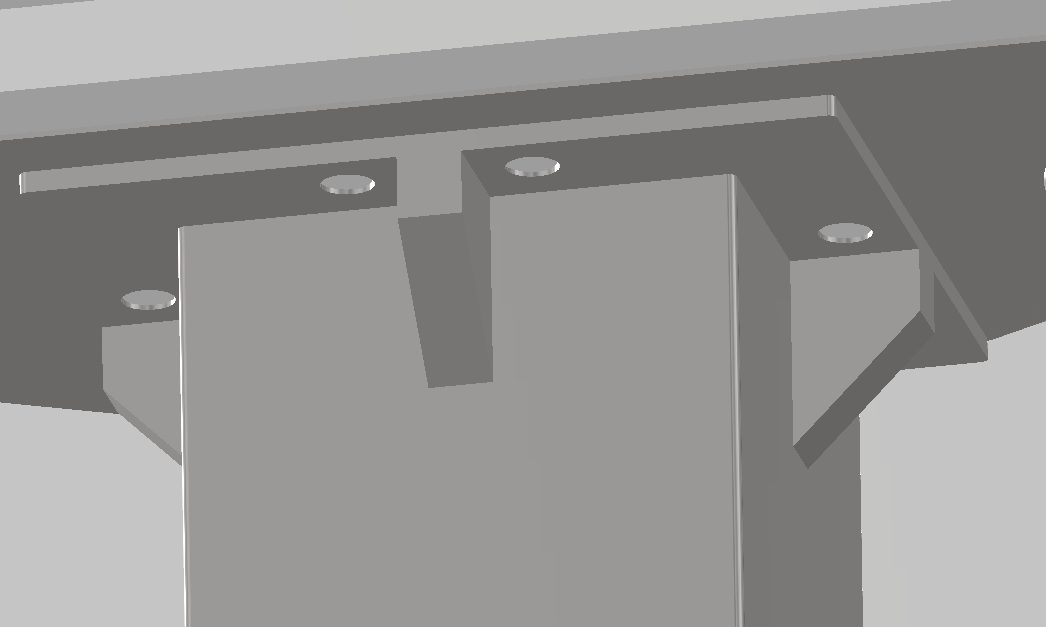
\includegraphics[width=0.8\linewidth,keepaspectratio]{media/image55.png}
  \caption{Refuerzos triangulares superiores en la conexión gabinete-poste.}
  \label{fig:refuerzos-sup}
  \fuente{Elaboración propia.}
\end{figure}

\textbf{Refuerzos triangulares inferiores} (Figura~\ref{fig:refuerzos-inf}): cuatro placas de acero A36 de 8~mm (350~mm, 23°, base 130~mm), una por cara. Transfieren el momento de vuelco a la cimentación, previenen el pandeo local en la base y, soldados al poste y a la placa base, conforman un empotramiento que hace trabajar al poste como viga en voladizo desde la base.

\begin{figure}[H]
  \centering
  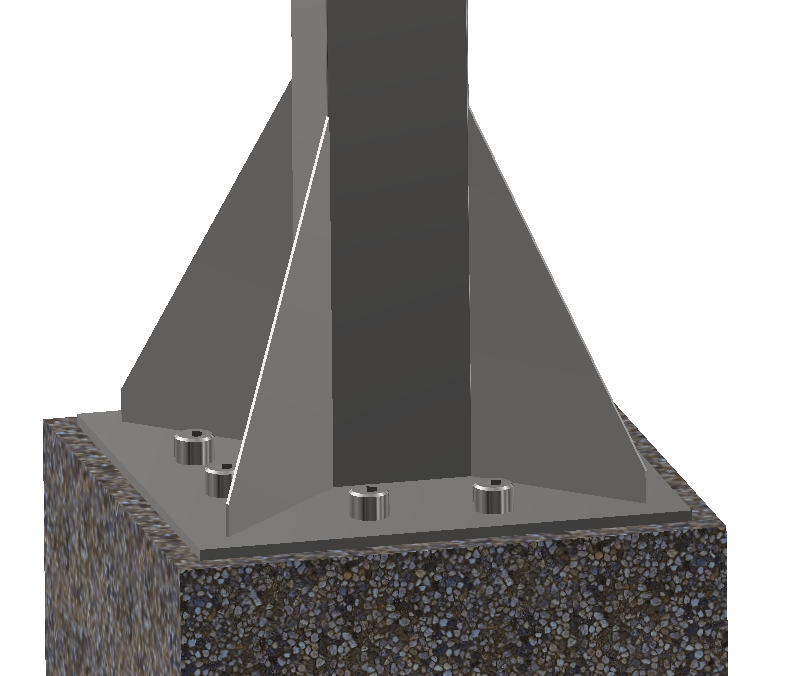
\includegraphics[width=0.8\linewidth,keepaspectratio]{media/image159.png}
  \caption{Refuerzos triangulares inferiores en la transición poste-zapata.}
  \label{fig:refuerzos-inf}
  \fuente{Elaboración propia.}
\end{figure}

\textbf{Zapata de cimentación} (Figuras~\ref{fig:zapata} y~\ref{fig:zapata-conexion}): hormigón armado de resistencia característica $f'_c = 210$~kg/cm\textsuperscript{2} (21~MPa), con geometría escalonada en dos niveles: pedestal de 500$\times$500~mm y 800~mm de altura, y zapata de 700$\times$700~mm y 350~mm de altura. La zapata distribuye las cargas concentradas del poste sobre el suelo y aporta masa para resistir el momento de vuelco sin levantar. El pedestal sobresale del terreno para evitar la acumulación de agua en la base. La interfaz aluminio-acero requiere aislamiento galvánico por la diferencia de potencial electroquímico entre ambos materiales; el poste se protege además mediante galvanización por inmersión en caliente (NTP-ISO) y pintura de poliuretano resistente a UV (120--150~µm), cumpliendo la normativa municipal MML.

\begin{figure}[H]
  \centering
  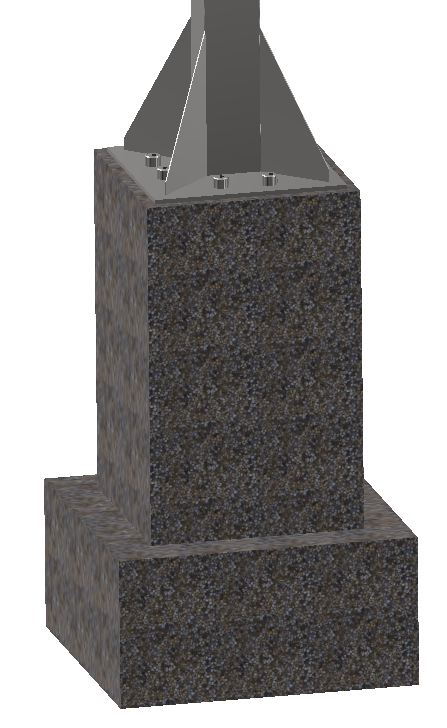
\includegraphics[width=0.8\linewidth,keepaspectratio]{media/image90.png}
  \caption{Zapata de cimentación de hormigón armado.}
  \label{fig:zapata}
  \fuente{Elaboración propia.}
\end{figure}

\begin{figure}[H]
  \centering
  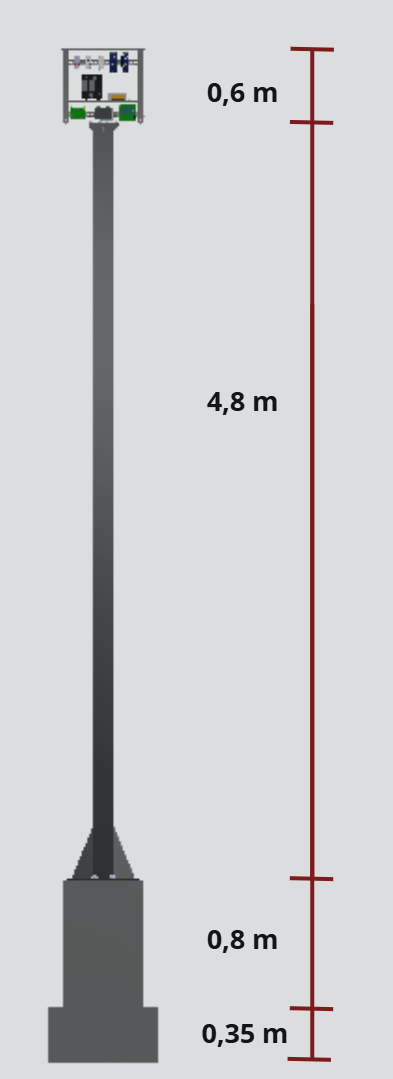
\includegraphics[width=0.8\linewidth,keepaspectratio]{media/image96.png}
  \caption{Detalle de la conexión entre el poste y la zapata de cimentación.}
  \label{fig:zapata-conexion}
  \fuente{Elaboración propia.}
\end{figure}

\section{Análisis estructural por elementos finitos}\label{sec:analisis-estructural}

Para validar el diseño estructural del conjunto (gabinete, rack, poste y zapata) bajo condiciones de servicio extremas, se realizó un análisis por elementos finitos (FEA) en Autodesk Inventor Professional, considerando cargas gravitatorias, cargas laterales de viento y condiciones de frontera representativas del sistema instalado.

\subsection{Condiciones de simulación y cargas aplicadas}\label{subsec:condiciones-fem}

El modelo incluye el gabinete de aluminio 5052-H32 (cubo hueco de 6~mm con refuerzos), el rack interno con la electrónica modelada como masas concentradas, el poste de acero A36 (130$\times$130$\times$10~mm, 4\,800~mm), los refuerzos triangulares superiores e inferiores, una placa base de 400$\times$400$\times$20~mm y el sistema de movimiento (aro, rodamiento, biela y conector). Las cargas gravitatorias incluyen el peso propio (calculado por el software), la masa del rack (11.965~kg) y la del sistema de movimiento (11.299~kg), con $g = 9.81$~m/s\textsuperscript{2} en $-Y$.

Las cargas de viento se basan en la NTE E.020 (SENCICO) complementada con AASHTO LRFD. La presión de viento de diseño normativa es de 1.0~kPa (velocidad $\approx 145$~km/h, periodo de retorno de 50 años); como supuesto conservador envolvente, la simulación aplica $q = 1.5$~kPa ($\approx 175$~km/h), perpendicular a las superficies frontales (600$\times$525~mm) y laterales (479$\times$525~mm) del gabinete. Las superficies inferiores de la placa base se restringieron en todos los grados de libertad, simulando la conexión rígida con la zapata.

\subsection{Tensiones de Von Mises}\label{subsec:von-mises}

La tensión de Von Mises es el criterio de falla más utilizado para materiales dúctiles, pues predice el inicio de la fluencia plástica. La tensión máxima del sistema, de \textbf{46.28~MPa}, se localiza en la transición entre el aro estructural del sistema de vigilancia y el poste (Figuras~\ref{fig:vm-completo} y~\ref{fig:vm-inferior}), debido a la discontinuidad geométrica entre el perfil cuadrado y la geometría circular del aro (Ø420~mm), que actúa como ménsula soportando cargas gravitatorias y laterales. Este valor está muy por debajo de los límites elásticos del aluminio 5052-H32 (193~MPa) y del acero A36 (250~MPa), confirmando operación en rango elástico. En el resto de la estructura las tensiones son bajas, con elevaciones locales en las esquinas de conexión y en las fijaciones de los componentes pesados del rack (UPS, SMPS).

\begin{figure}[H]
  \centering
  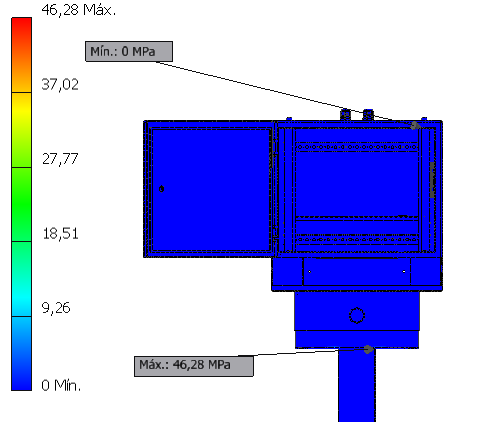
\includegraphics[width=0.8\linewidth,keepaspectratio]{media/image134.png}
  \caption{Distribución de tensión de Von Mises en el sistema completo.}
  \label{fig:vm-completo}
  \fuente{Elaboración propia.}
\end{figure}

\begin{figure}[H]
  \centering
  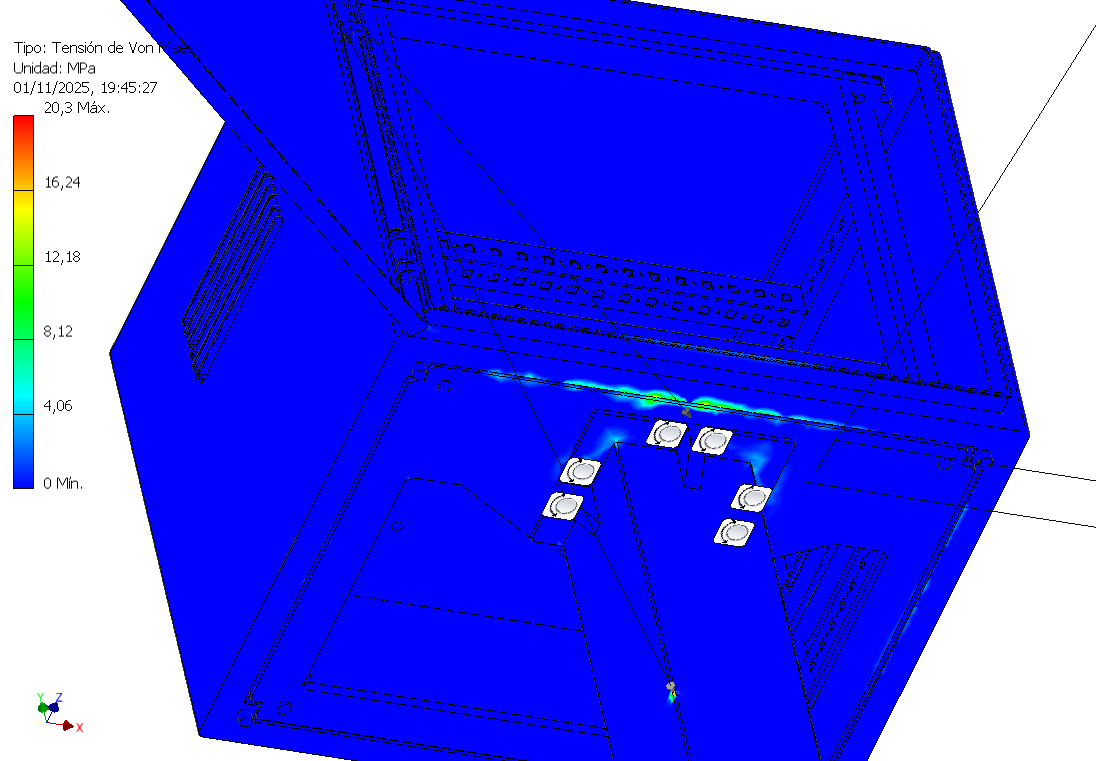
\includegraphics[width=0.8\linewidth,keepaspectratio]{media/image31.png}
  \caption{Tensión de Von Mises, vista inferior del gabinete.}
  \label{fig:vm-inferior}
  \fuente{Elaboración propia.}
\end{figure}

\subsection{Tensiones principales}\label{subsec:tensiones-principales}

La primera tensión principal ($\sigma_1$, tracción máxima) alcanza \textbf{39.63~MPa} en la interfaz aro-poste, con una compresión complementaria de $-18.59$~MPa en el lado opuesto, comportamiento típico de flexión (Figura~\ref{fig:tension-p1}). La tercera tensión principal ($\sigma_3$, compresión máxima) alcanza \textbf{$-70.52$~MPa} en la cara frontal de la misma conexión, con una tracción máxima de 15.36~MPa en la base frontal del rack (Figura~\ref{fig:tension-p3}). Los 39.63~MPa de tracción representan el 20.5~\% del límite elástico del aluminio, y los $-70.52$~MPa de compresión, el 36.5~\% del mismo, confirmando amplia reserva sin plastificación bajo la carga extrema de 175~km/h.

\begin{figure}[H]
  \centering
  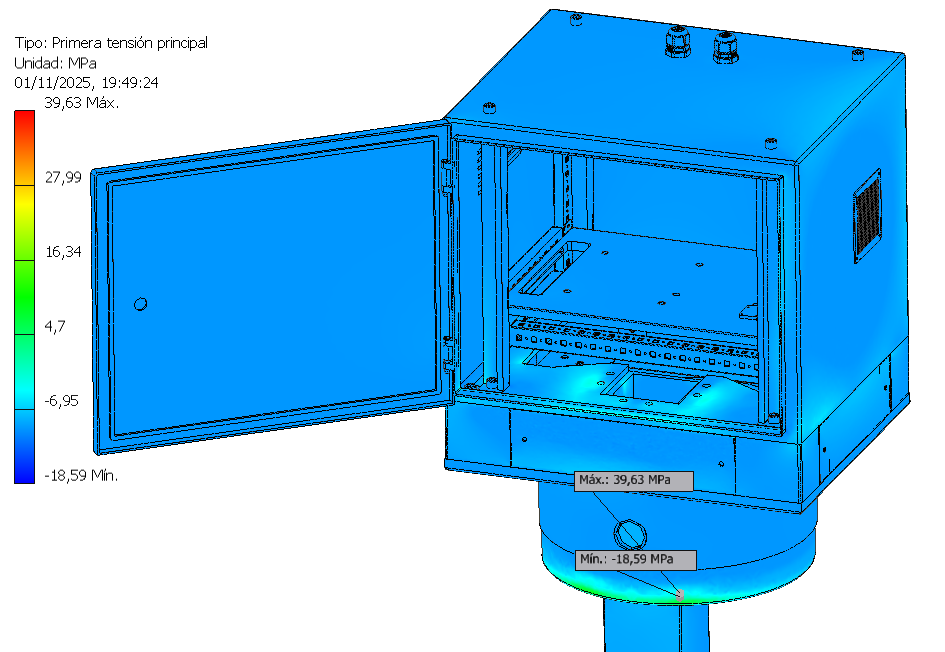
\includegraphics[width=0.8\linewidth,keepaspectratio]{media/image100.png}
  \caption{Distribución de la primera tensión principal.}
  \label{fig:tension-p1}
  \fuente{Elaboración propia.}
\end{figure}

\begin{figure}[H]
  \centering
  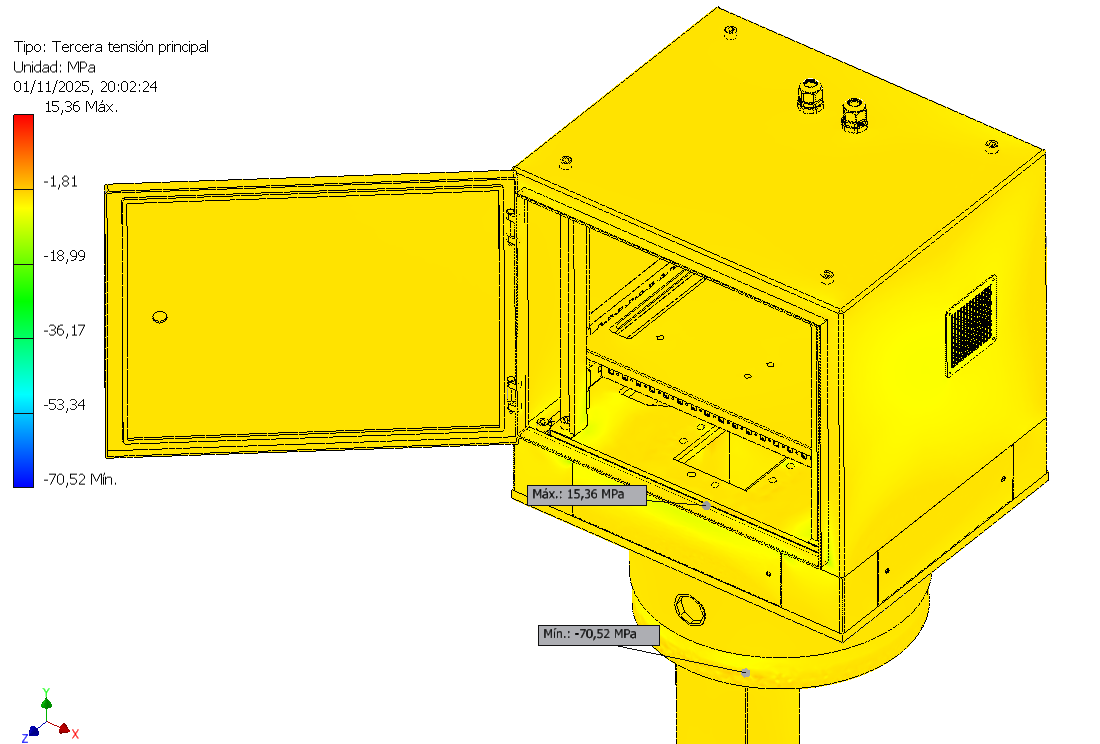
\includegraphics[width=0.8\linewidth,keepaspectratio]{media/image141.png}
  \caption{Distribución de la tercera tensión principal.}
  \label{fig:tension-p3}
  \fuente{Elaboración propia.}
\end{figure}

Se verifica además el pandeo local del perfil tubular. La relación ancho-espesor del perfil 130$\times$130$\times$10~mm es $\lambda = b/t = 13$, inferior al límite de sección compacta según AISC:

\begin{equation}
\lambda_p = 1.12\sqrt{E/f_y} = 1.12\sqrt{200\,000/250} \approx 31.7
\end{equation}

Como $\lambda = 13 < \lambda_p = 31.7$, el perfil se clasifica como sección compacta: alcanzará el límite elástico antes de pandear localmente, por lo que el criterio de falla relevante es la fluencia. El factor de seguridad respecto a la compresión máxima es $FS = 250/70.52 = 3.545$, es decir, la compresión representa solo el 28.2~\% del límite elástico del acero A36.

\subsection{Desplazamientos}\label{subsec:desplazamientos}

El campo de desplazamientos (Figuras~\ref{fig:desplazamiento-total} y~\ref{fig:desplazamiento-gabinete}) presenta un gradiente progresivo desde la base empotrada (0~mm) hasta las esquinas superiores del gabinete, con un desplazamiento máximo de \textbf{0.2103~mm} en la zona lateral del gabinete. Este valor es prácticamente imperceptible y se produce bajo la carga de viento extrema de 1.5~kPa (175~km/h). Bajo la presión de diseño nominal de 1.0~kPa (145~km/h, retorno de 50 años) los desplazamientos se reducirían proporcionalmente a $\approx 0.14$~mm, deflexión completamente imperceptible que confirma la rigidez del conjunto.

\begin{figure}[H]
  \centering
  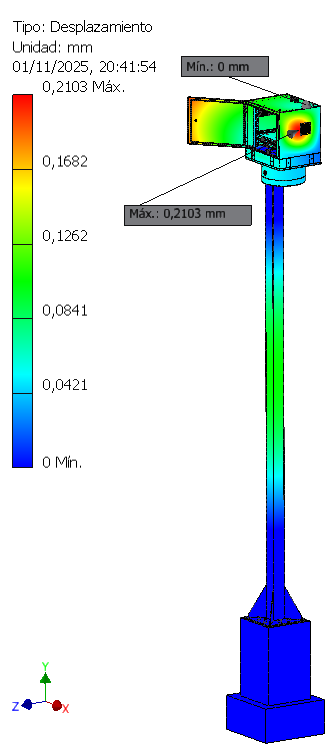
\includegraphics[width=0.8\linewidth,keepaspectratio]{media/image61.png}
  \caption{Campo de desplazamientos totales del sistema.}
  \label{fig:desplazamiento-total}
  \fuente{Elaboración propia.}
\end{figure}

\begin{figure}[H]
  \centering
  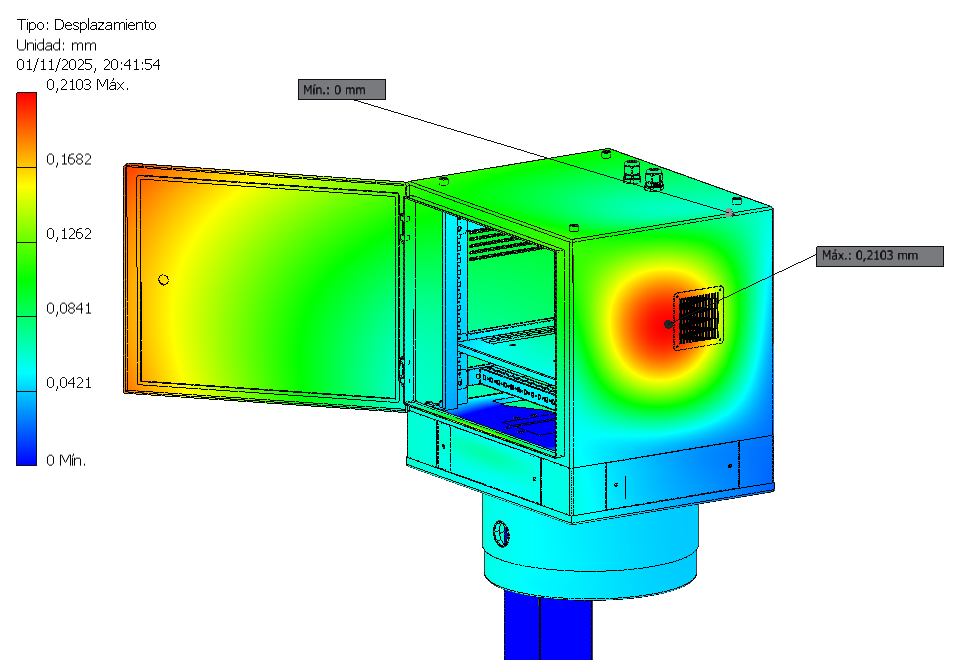
\includegraphics[width=0.8\linewidth,keepaspectratio]{media/image99.png}
  \caption{Desplazamientos en el gabinete.}
  \label{fig:desplazamiento-gabinete}
  \fuente{Elaboración propia.}
\end{figure}

\subsection{Factor de seguridad}\label{subsec:factor-seguridad}

El factor de seguridad calculado por el software (Figuras~\ref{fig:fs-sistema} y~\ref{fig:fs-gabinete}) es $\geq 15$ en prácticamente todo el sistema (gabinete, rack y poste), con un \textbf{mínimo de 5.94} localizado en la transición entre el aro del sistema de vigilancia y el poste. Esta reducción local se debe a la concurrencia de la discontinuidad geométrica (perfil cuadrado a aro circular), la carga en voladizo del sistema de visión y la presión lateral de viento sobre el aro. Aun siendo el punto más esforzado, un factor de 5.94 es satisfactorio y conservador para equipamiento urbano: supera el mínimo de 3.0 recomendado para estructuras metálicas sometidas a fatiga por viento, compensa las incertidumbres del modelo FEA (tolerancias de fabricación, homogeneidad del material, calidad de soldaduras) y aporta robustez ante cargas dinámicas no modeladas (ráfagas impulsivas, vibraciones de tráfico, impactos de mantenimiento), garantizando una vida útil superior a 15 años.

\begin{figure}[H]
  \centering
  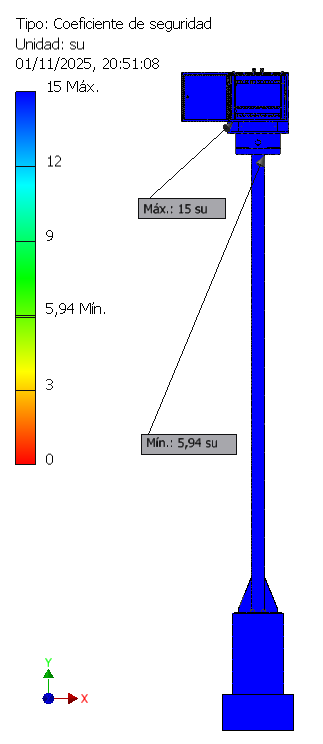
\includegraphics[width=0.8\linewidth,keepaspectratio]{media/image130.png}
  \caption{Distribución del factor de seguridad en el sistema.}
  \label{fig:fs-sistema}
  \fuente{Elaboración propia.}
\end{figure}

\begin{figure}[H]
  \centering
  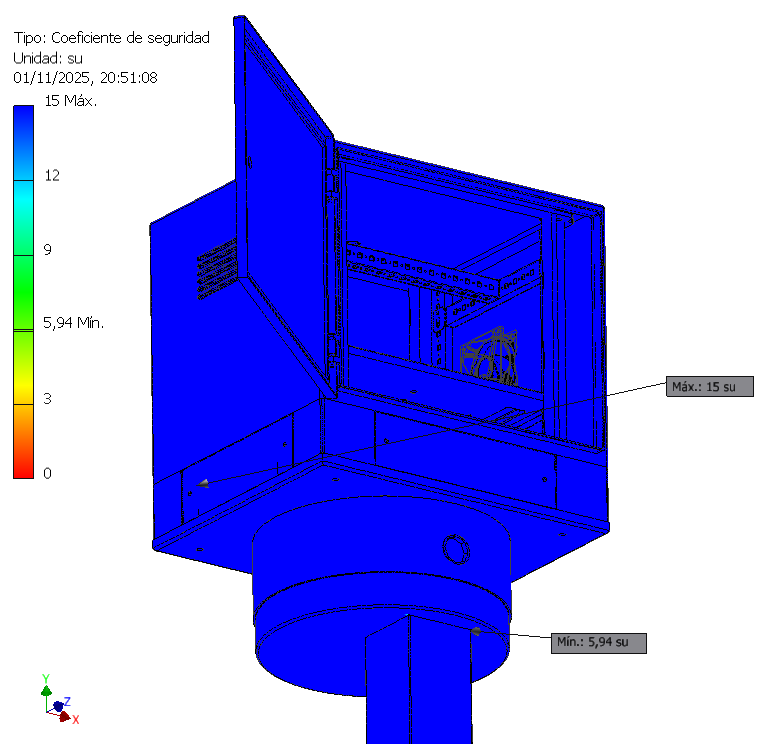
\includegraphics[width=0.8\linewidth,keepaspectratio]{media/image1.png}
  \caption{Factor de seguridad enfocado en el gabinete.}
  \label{fig:fs-gabinete}
  \fuente{Elaboración propia.}
\end{figure}

\section{Análisis térmico}\label{sec:analisis-termico}

El análisis térmico verifica que la temperatura interna del gabinete permanezca dentro de los límites operativos de los componentes. Los más sensibles (Raspberry~Pi~5, HAT~4G~LTE) admiten 70--85\,°C, mientras que los de potencia (SMPS, UPS, driver) toleran hasta 105\,°C en puntos calientes internos.

\subsection{Generación de calor y ventilación}\label{subsec:generacion-calor}

La potencia disipada como calor proviene de las pérdidas de conversión y del consumo de los componentes. Las contribuciones estimadas son: SMPS S-360-24 (eficiencia 85~\%) con $P_{\text{out}} = 24 \times 15 = 360$~W y pérdidas $P = 360(1-0.85)/0.85 = 63.5$~W; UPS 500\,VA en recarga, $500 \times 0.08 = 40$~W; driver DM542T (eficiencia 90~\%), con $P_{\text{motor}} = 24 \times 3 \times 2 = 144$~W y pérdidas $144(1-0.90)/0.90 = 16$~W; Raspberry~Pi~5, 15~W; HAT~4G~LTE, 5~W; y conversores DC-DC (eficiencia 85~\%), $(5\times3 + 12\times2)\times0.15/0.85 = 8.4$~W. La potencia térmica total a evacuar es:

\begin{equation}
Q_{\text{total}} = 63.5 + 40 + 16 + 15 + 5 + 8.4 = 147.9~\text{W} \approx 150~\text{W}
\end{equation}

Para evacuar estos 150~W se implementa ventilación forzada mediante un ventilador axial de 120$\times$120$\times$38~mm (24~V~DC, 12~W, caudal nominal 180~m\textsuperscript{3}/h $= 0.05$~m\textsuperscript{3}/s, presión estática 80~Pa) ubicado en la parte superior del gabinete, con ingreso de aire fresco por rejillas inferiores frontales con filtro de polvo lavable (Figura~\ref{fig:ventilador}). El incremento de temperatura del aire al atravesar el gabinete se obtiene por balance térmico $Q = \dot{m}\,c_p\,\Delta T$, con $\rho_{\text{aire}} = 1.2$~kg/m\textsuperscript{3}, $c_p = 1\,005$~J/(kg·K) y caudal de 0.05~m\textsuperscript{3}/s:

\begin{equation}
\dot{m} = \rho_{\text{aire}} \times V = 1.2 \times 0.05 = 0.06~\text{kg/s}
\end{equation}
\begin{equation}
\Delta T = \frac{Q}{\dot{m}\,c_p} = \frac{150}{0.06 \times 1\,005} = \frac{150}{60.3} = 2.5~^\circ\text{C}
\end{equation}

El aire se calienta solo 2.5\,°C al atravesar el gabinete a caudal nominal. En el caso más desfavorable de temperatura ambiente de 60\,°C, el aire expulsado alcanzaría $\approx 62.5$\,°C y la temperatura interna promedio se mantendría en torno a 61\,°C, dentro del rango operativo de todos los componentes.

\begin{figure}[H]
  \centering
  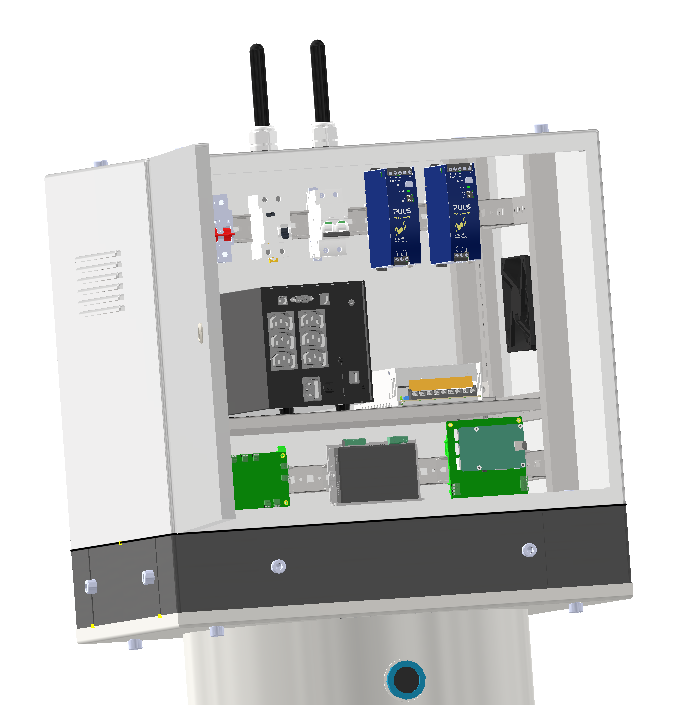
\includegraphics[width=0.8\linewidth,keepaspectratio]{media/image29.png}
  \caption{Vista del ventilador y la salida de aire caliente del gabinete.}
  \label{fig:ventilador}
  \fuente{Elaboración propia.}
\end{figure}

\subsection{Plan de validación experimental}\label{subsec:validacion-termica}

El balance térmico anterior es un modelo conservador de flujo estacionario; su confirmación definitiva se realizará mediante ensayos físicos del prototipo, que constituyen el trabajo experimental previsto. Se ejecutará un ensayo en cámara climática reproduciendo el rango normativo de $-20$\,°C a $+60$\,°C, instrumentando el interior del gabinete con termopares en los puntos calientes (SMPS, UPS, driver y Raspberry~Pi~5) para registrar el $\Delta T$ real y contrastarlo con los 2.5\,°C calculados. Se incorporará una fuente de radiación solar simulada que reproduzca la irradiancia máxima de Lima sobre las caras expuestas del gabinete, evaluando el efecto del anodizado y la carga térmica adicional sobre la temperatura interna. Finalmente, se someterá el conjunto a ciclos térmicos repetidos entre los extremos del rango operativo para verificar la estabilidad de los sellos IP65, la ausencia de condensación interna y el correcto accionamiento de la ventilación forzada a 40\,°C, así como la integridad de las juntas tras el envejecimiento por fatiga térmica. Los resultados de estos ensayos permitirán ajustar, de ser necesario, el caudal del ventilador o la disposición de las rejillas de admisión.

\section{Listado consolidado de planos mecánicos}\label{sec:planos-mecanicos}

El diseño mecánico se documenta mediante un conjunto de planos técnicos organizados por subsistema, cuyo detalle dimensional, de tolerancias y de materiales se presenta en el Anexo de planos. Los planos generados son los siguientes:

\begin{enumerate}
  \item \textbf{Gabinete de aluminio 5052-H32:} geometría de cubo hueco, espesores de pared, rejillas de ventilación, sellos y puntos de fijación al rack.
  \item \textbf{Rack interno de soporte:} perfiles de 30$\times$30~mm, bandejas perforadas, rieles DIN y distribución vertical de componentes en los cuatro niveles funcionales.
  \item \textbf{Soporte de movimiento de la cámara:} aro estructural giratorio, rodamiento de Ø120~mm, biela, conector cámara-biela y montaje del motor NEMA~23.
  \item \textbf{Poste y soporte del controlador semafórico:} perfil tubular de acero A36 (130$\times$130$\times$10~mm), refuerzos triangulares superiores e inferiores y placa base.
  \item \textbf{Zapata de cimentación:} geometría escalonada (pedestal y zapata), armadura de refuerzo y detalle de anclaje del poste.
\end{enumerate}

El conjunto de planos garantiza la trazabilidad entre los cálculos y las verificaciones de este capítulo y la fabricación e instalación del sistema en campo.
